% ~ 6 pages
\chapter{The ATLAS Experiment at the Large Hadron Collider}
\label{chap:atlas}

The ATLAS experiment is located at the LHC at CERN, a symmetric proton--proton
and heavy ion collider, supplying collision events to four major experiments. In
proton--proton operation, bunches of protons are crossed at the interaction
points located inside of the experiments with a peak bunch crossing rate
of~\SI{40}{\mega\hertz}~\cite{lhc}. With a proton beam energy of \SI{6.5}{\TeV}
during Run~2 of the LHC, the proton--collisions take place at a center-of-mass
energy of \SI{13}{\TeV}. During the 2016 data taking period, a peak
instantaneous luminosity of~\SI{1.4e34}{\per\square\centi\metre\per\second} was
reached~\cite{lhc_2016_report}, which was further increased during the 2017 data
taking period.

\section{Overview of the ATLAS Detector}
\label{sec:atlas}

The ATLAS detector, described in Ref.\ \cite{atlas_detector}, is a multipurpose
particle detector experiment. An overview of the detector is given in
Figure~\ref{fig:atlas_detector}. Its cylindrical geometry provides almost
$4\pi$~coverage and forward-backward symmetry with respect to the nominal
interaction point. Specialised detector subsystems are arranged in concentric
layers around the beam axis, enabling the reconstruction of photons, electrons,
muons, taus and jets. Moreover, the detector coverage allows to reconstruct
missing transverse energy from weakly and non-interacting particles.

\begin{figure}[htb]
  \centering
  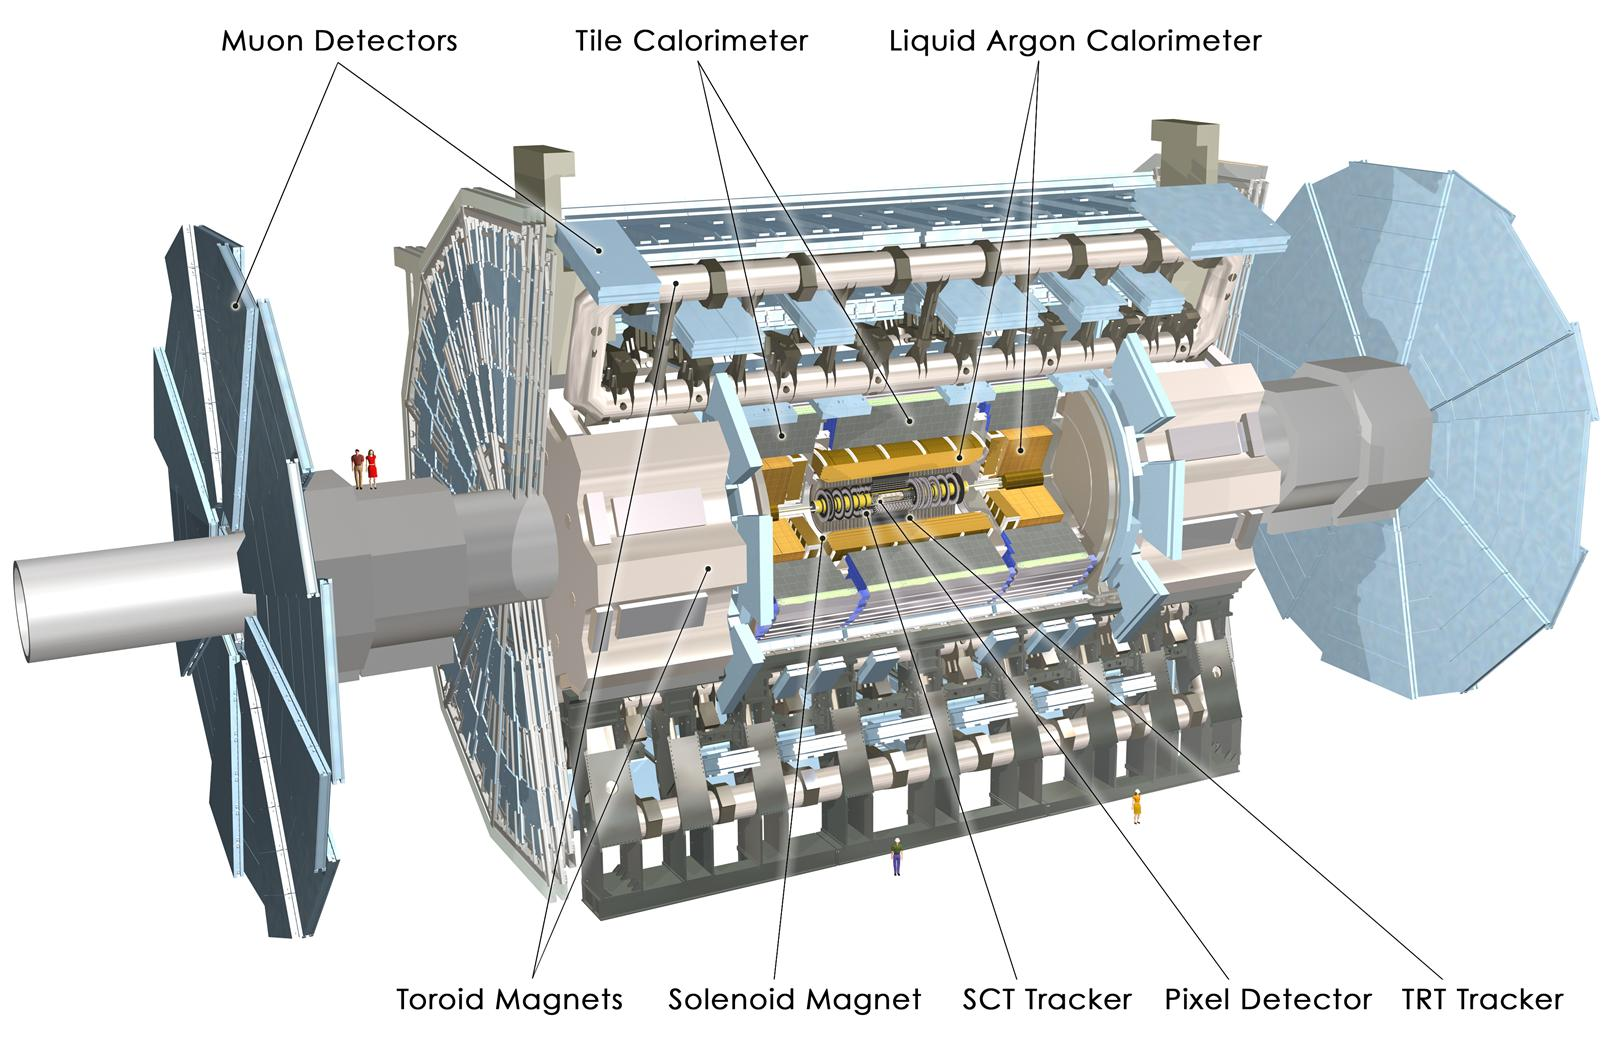
\includegraphics[width=0.8\textwidth]{./figures/atlas/overview.jpg}
  \caption[Overview of the ATLAS detector]{Overview of the ATLAS
    detector~\cite{atlas_detector}. Shown is the inner detector consisting of
    pixel, microstrip (SCT), transition radiation tracker (TRT) and solenoid;
    the calorimeter system consisting of LAr and Tile sampling calorimeters and
    the muon spectrometer consisting of tracking chambers and air-core toroids.}
  \label{fig:atlas_detector}
\end{figure}

In the ATLAS experiment a right-handed coordinate system is used to describe
positions in the detector. The origin of the coordinate system is located at the
nominal interaction point, with the $z$-axis pointing along the beam axis, the
$x$-axis towards the centre of the LHC ring and the $y$-axis upwards. The $x$-
and $y$-axes span the transverse plane. Spherical
coordinates~$(r, \varphi, \theta)$ are commonly used, with the azimuthal
angle~$\varphi$ being measured in the transverse plane and the polar
angle~$\theta$ with respect to the beam axis.

Due to the unknown longitudinal momentum of colliding partons in the
proton--proton collisions, the momentum of final state particles only balances
in the transverse plane. Therefore, transverse quantities for momentum and
energy are defined as
\begin{align*}
  p_\text{T} &= |\mathbf{p}| \sin\theta & E_\text{T} &= E \sin\theta \eqdot
\end{align*}
In addition, the unknown boost along the $z$-axis motivates the definition of
the pseudorapidity
\begin{align*}
  \eta &= -\ln\left[ \tan\left( \frac{\theta}{2} \right) \right] \eqcomma
\end{align*}
such that differences in~$\eta$ are Lorentz-invariant in the massless limit, and
the angular distance
\begin{align*}
  \Delta R &= \sqrt{\left(\Delta\eta\right)^2 + \left(\Delta\varphi\right)^2} \eqcomma
\end{align*}
where $\Delta \eta$ and $\Delta \varphi$ are the differences in pseudorapidity
and azimuthal angle, respectively.

In the following a brief description of the detector subsystems is given. In
increasing radial distance from the beam axis, the systems are:
\begin{description}
\item[Inner Detector] The inner detector (ID) consists of several layers of
  pixel detectors, silicon microstrip detectors and straw chambers. The ID is
  embedded in a \SI{2}{\tesla} axial magnetic field, bending the trajectories of
  charged particles in the transverse plane, thus allowing transverse momentum
  measurements. Hits of charged tracks in the active layers of the ID are
  reconstructed as so called space points, which are used to perform tracking
  and vertexing. The straw tubes of the Transition Radiation Tracker (TRT) offer
  tracking at large radii as well as electron identification via high-threshold
  hits originating from transition radiation of electrons crossing the polymer
  material between the straws.

\item[Calorimeter System] The sampling calorimeters used in the ATLAS detector
  allow to measure the energies of photons, electrons and hadrons. The
  calorimeter system consists of an electromagnetic calorimeter with high
  granularity, designed to reconstruct energy depositions of photons and
  electrons, and the coarser hadronic calorimeter to reconstruct jets of
  hadrons.

\item[Muon Spectrometer] Muons passing the calorimeter are measured in
  high-precision tracking chambers in the magnetic field of an air-core toroid.
  The spectrometer allows to identify muons and measure their momentum from the
  curvature of reconstructed tracks in the muon system.

\item[Trigger and Data Acquisition Systems] The peak event rate of
  \SI{40}{\mega\hertz} in the ATLAS detector, mostly consisting of events not of
  immediate interest for physics research, needs to be reduced in a trigger
  system to match the limited throughput of the data acquisition systems, while
  still being sensitive to rare physics processes. The trigger of the ATLAS
  detector is divided into three levels: L1, L2 and the event filter. They
  successively reduce the rate, while having access to detector information of
  increasing granularity. After the final trigger level, the event filter, the
  rate is sufficiently small, such that events can be moved to permanent storage
  for later analysis.
\end{description}
For the reconstruction of hadronic tau decays, the tracking and calorimeter
systems are of large importance. In the following they are described in more
detail.

\section{The Inner Detector}
\label{sec:atlas_tracking}

The inner detector of the ATLAS experiment provides track reconstruction in the
high particle density environment of proton--proton collisions at the LHC. The
tracking system meets the transverse momentum and vertex resolution requirements
needed to perform physics analyses. An overview of the inner detector is shown
in Figure~\ref{fig:atlas_indet}.

\begin{figure}[htb]
  \centering
  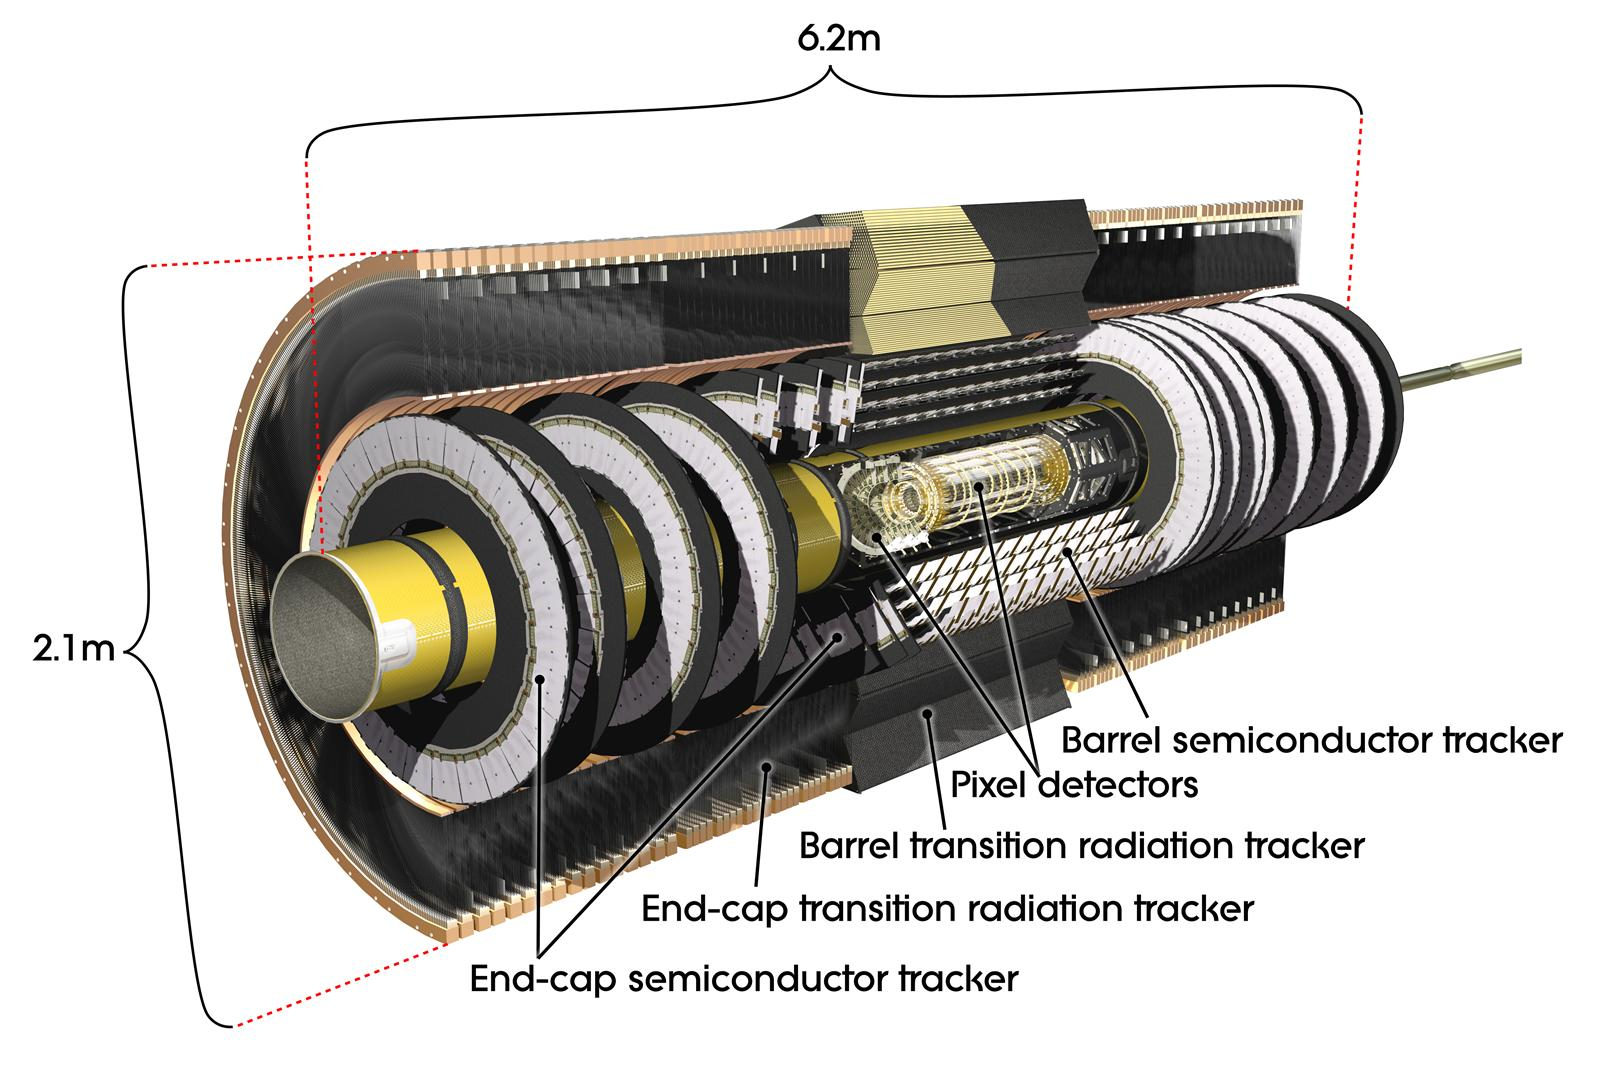
\includegraphics[width=0.75\textwidth]{./figures/atlas/inner_detector.jpg}
  \caption[Overview of the ATLAS inner detector]{Overview of the ATLAS inner
    detector~\cite{indet_fig}. Shown are pixel and microstrip detector as well
    as the Transition Radiation Tracker. The innermost pixel layer, the
    Insertable B-Layer, is not depicted.}
  \label{fig:atlas_indet}
\end{figure}

The inner detector consists of three distinct and complementary parts employing
different detector technologies. From the interaction point outwards, it
consists of: pixel detectors, silicon microstrip detectors and a transition
radiation detector using drift tubes.

The pixel detectors consist of the Insertable B-Layer (IBL), installed during
Long~Shutdown~1 at a reduced distance from the interaction point
of~$r = \SI{33.25}{\milli\metre}$~\cite{ibl_tdr}, and three additional layers
spanning radial distances from \SI{50.5}{\milli\metre} to
\SI{122.5}{\milli\metre}~\cite{atlas_detector} in the barrel of the ATLAS
detector. Additionally, three disks of pixel detectors cover the forward and
backward regions in two endcaps. The sensors of the IBL provide an intrinsic
resolution of approximately \SI{10}{\micro\metre} in the azimuthal ($r\varphi$)
direction and \SI{65}{\micro\metre} in $z$-direction~\cite{ibl_measurement}. The
other pixel layers have resolutions of \SI{10}{\micro\metre} in $r\varphi$ and
\SI{115}{\micro\metre} in $z$-direction~\cite{atlas_detector}. The high
resolution of the pixel detectors and their proximity to the interaction point
are crucial for track impact parameter measurements (cf.\
Figure~\ref{fig:impact_params}) and for primary as well as secondary vertex
reconstruction.

\begin{figure}[htb]
  \begin{subfigure}[t]{0.48\textwidth}
    \centering
    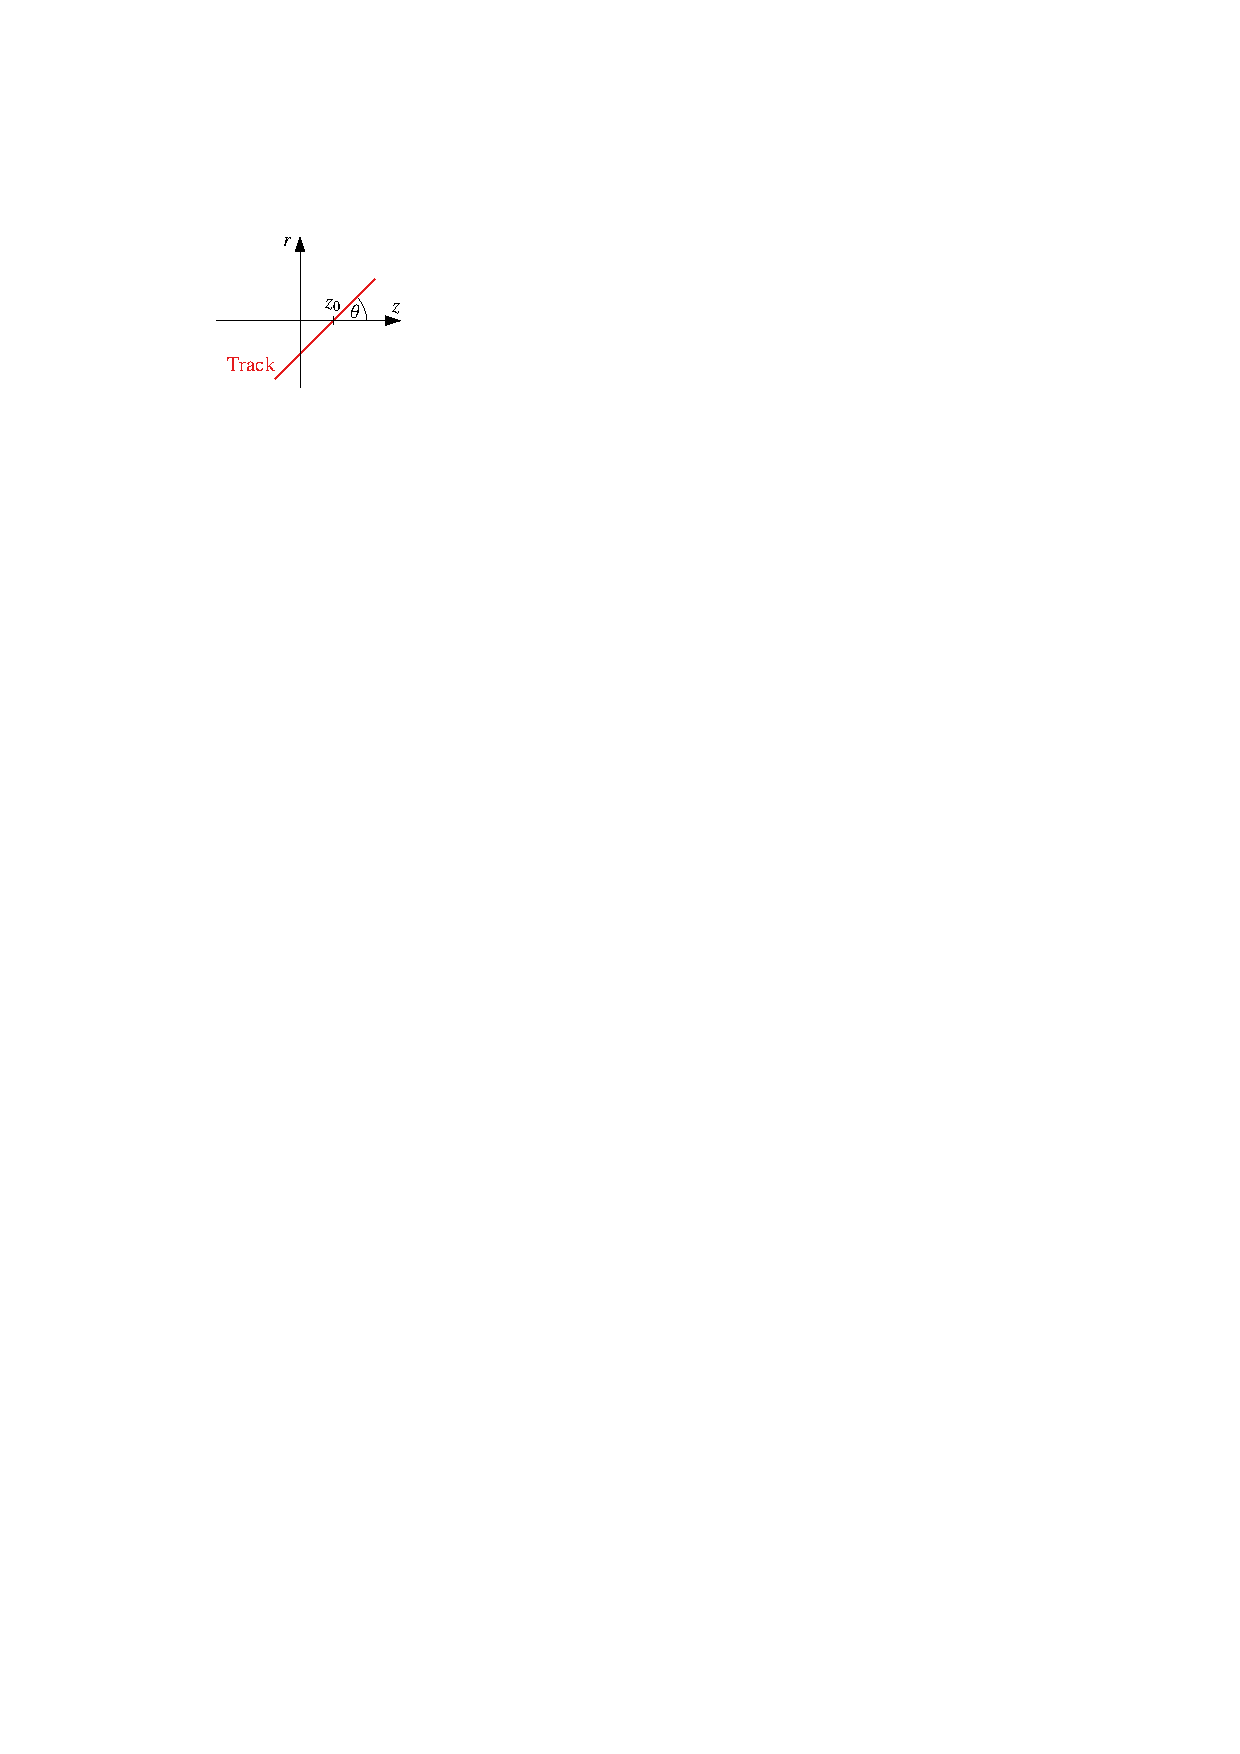
\includegraphics{./figures/atlas/impact_params_z0.pdf}
    \subcaption{Definition of the longitudinal impact parameter, $z_0$.}
    \label{fig:longitudinal_impact_param}
  \end{subfigure}\hfill
  \begin{subfigure}[t]{0.48\textwidth}
    \centering 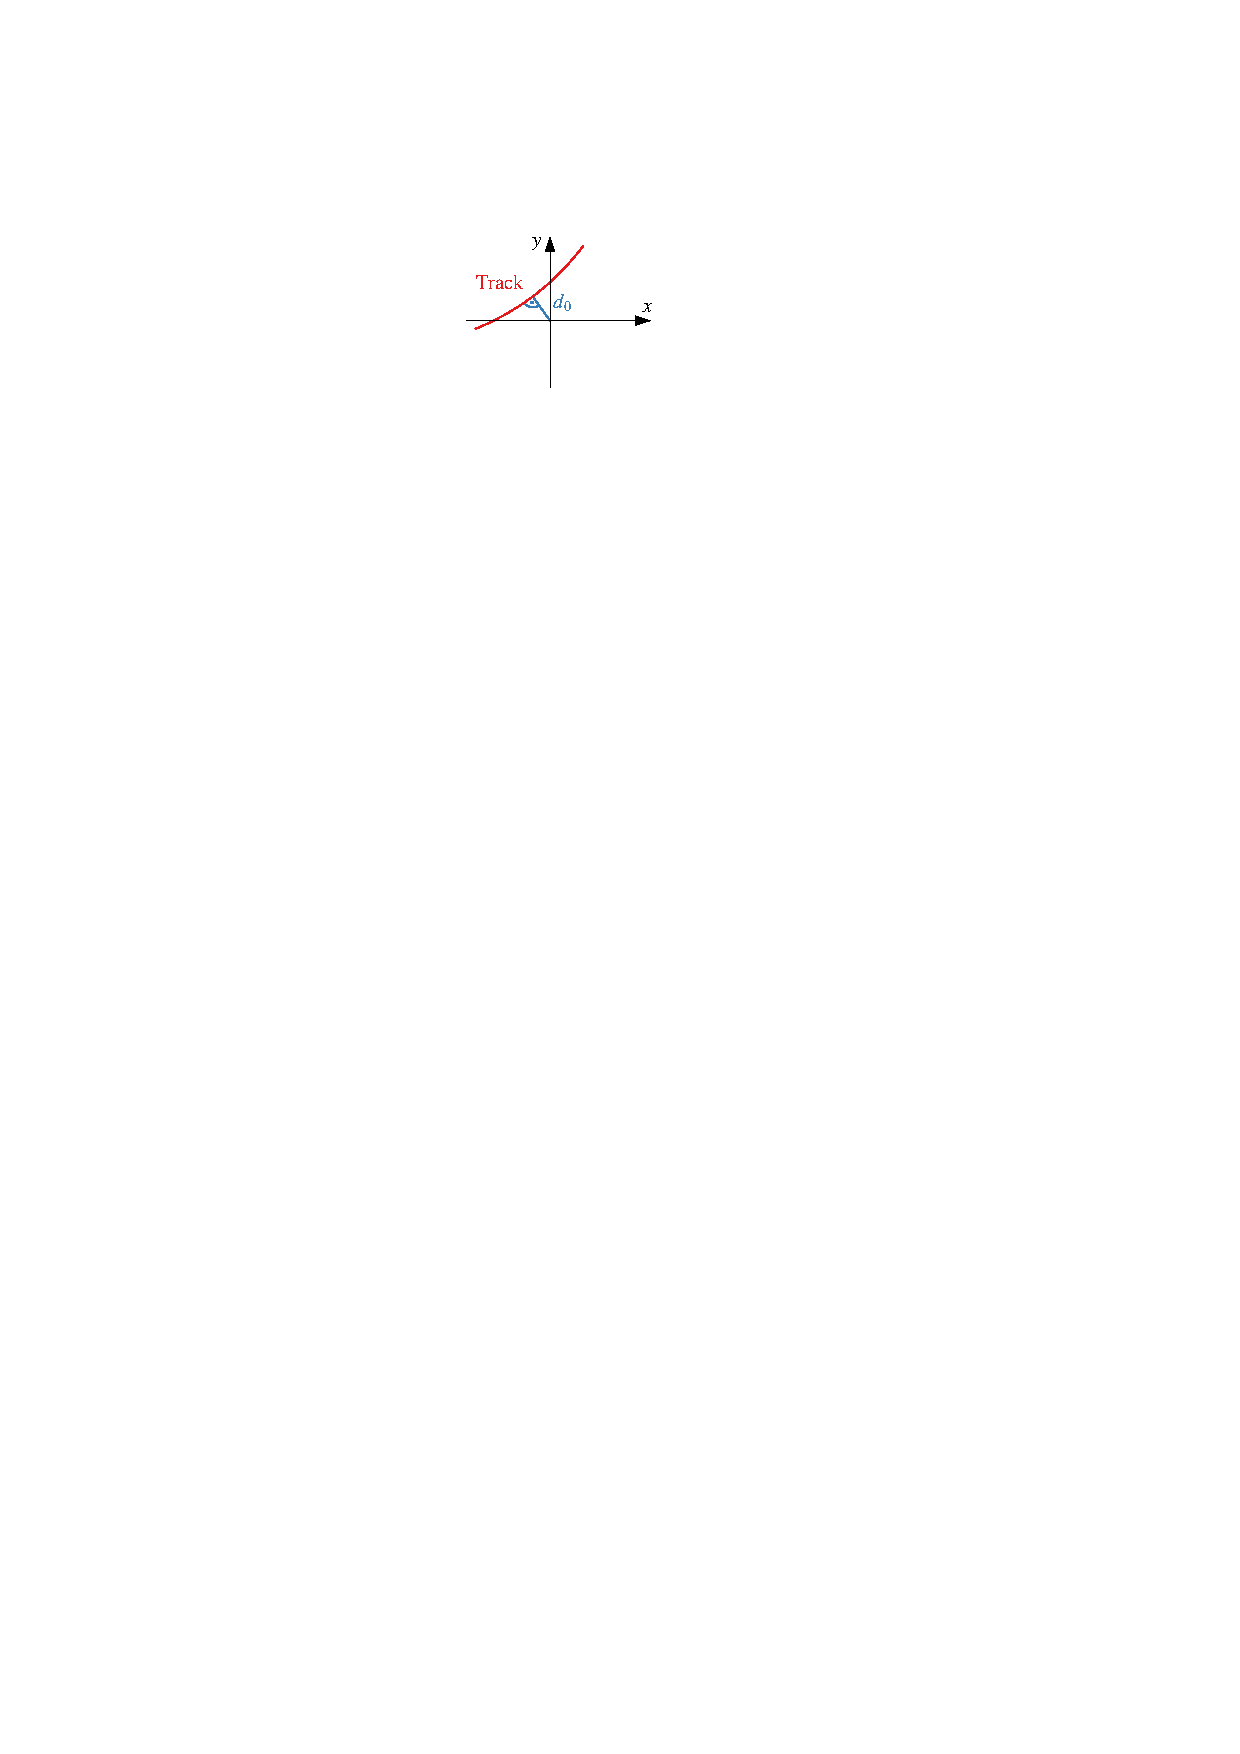
\includegraphics{./figures/atlas/impact_params_d0.pdf}
    \subcaption{Definition of the transverse impact parameter, $d_0$. The sign
      of $d_0$ depends on the angular momentum of the track w.r.t.\ the origin.}
    \label{fig:transverse_impact_param}
  \end{subfigure}
  \caption[Definition of track impact parameters]{Definition of track impact
    parameters at the perigee with respect to the origin.}
  \label{fig:impact_params}
\end{figure}

The Semiconductor Tracker (SCT) is a silicon microstrip detector with four
barrel layers covering the intermediate radial range from
$r = \SI{299}{\milli\metre}$ to \SI{514}{mm}~\cite{atlas_detector}. In the
endcaps, the SCT consists of nine disks perpendicular to the beam axis. The
intrinsic resolution of the SCT sensors is \SI{17}{\micro\metre} in $r\varphi$
and \SI{580}{\micro\metre} in axial (radial) direction for the barrel
(disks)~\cite{atlas_detector}. The semiconductor tracking detectors provide a
pseudorapidity coverage of approximately~$|\eta| < 2.5$.

Track measurement at large radial ranges of $r = \SI{554}{\milli\metre}$ to
\SI{1082}{\milli\metre} are provided by the TRT consisting of drift tubes with a
diameter of \SI{4}{\milli\metre} aligned with the beam
axis~\cite{atlas_detector}. As a result, they only provide azimuthal
measurements with an intrinsic resolution of
\SI{130}{\micro\metre}~\cite{atlas_detector}. With a large number of 73 (160)
straw planes in the barrel (endcap) it provides tracking and electron
identification over a pseudorapidity range
of~$|\eta| < 2.0$~\cite{atlas_detector}.

Charged-particle tracks are reconstructed from space points using sophisticated
pattern-recognition and tracking algorithms. After reconstruction, several
representations can be used to define tracks. In the ATLAS detector, tracks are
often represented at the perigee with respect to a reference point, which is
commonly the primary vertex or the beamspot. In this representation tracks are
unambiguously defined by the transverse and longitudinal impact parameters,
$d_0$ and $z_0$ (cf.\ Figure~\ref{fig:impact_params}), the azimuthal and polar
angles of the track momentum vector at the perigee, $\varphi$ and $\theta$, as
well as the ratio of charge and momentum of the track, $q / p$.

% See \url{https://twiki.cern.ch/twiki/bin/view/AtlasProtected/InDetTrackingDC14#Impact_parameters_z0_d0_definiti}

\section{The Calorimeter System}
\label{sec:atlas_calo}

The ATLAS calorimeter system employs sampling calorimeters to measure the energy
depositions of charged and neutral particles in the calorimeter material. It
provides a pseudorapidity coverage
of~\mbox{$|\eta| < 4.9$}~\cite{atlas_detector}. The calorimeter is divided into
two parts, the electromagnetic (EM) and the hadronic calorimeter, which are
further subdivided into samplings of varying thickness and granularity, thus
allowing the measurement of longitudinal and transverse shower shapes. The EM
calorimeter has a thickness of 22 to 24 radiation lengths\footnote{The radiation
  length~$X_0$ is the mean distance a high-energy electron passes through
  matter, until it loses all but~$e^{-1}$ of its initial energy due to
  bremsstrahlung.} depending on the detector region~\cite{atlas_detector}.
Typically, the EM calorimeter fully contains electromagnetic showers originating
from electrons and photons. The combined thickness of EM and hadronic
calorimeter is approximately ten interaction lengths\footnote{The interaction
  length~$\lambda$ is the mean distance a high-energy hadron passes through
  matter, until it performs an inelastic collision with a
  nucleon.}~\cite{atlas_detector}. Therefore, the calorimeters fully contain the
showers of most hadrons, minimising punch-through into the muon spectrometer and
allowing to reconstruct the missing transverse energy. An overview of the
calorimeter system is shown in Figure~\ref{fig:atlas_calo}.

\begin{figure}[htb]
  \centering
  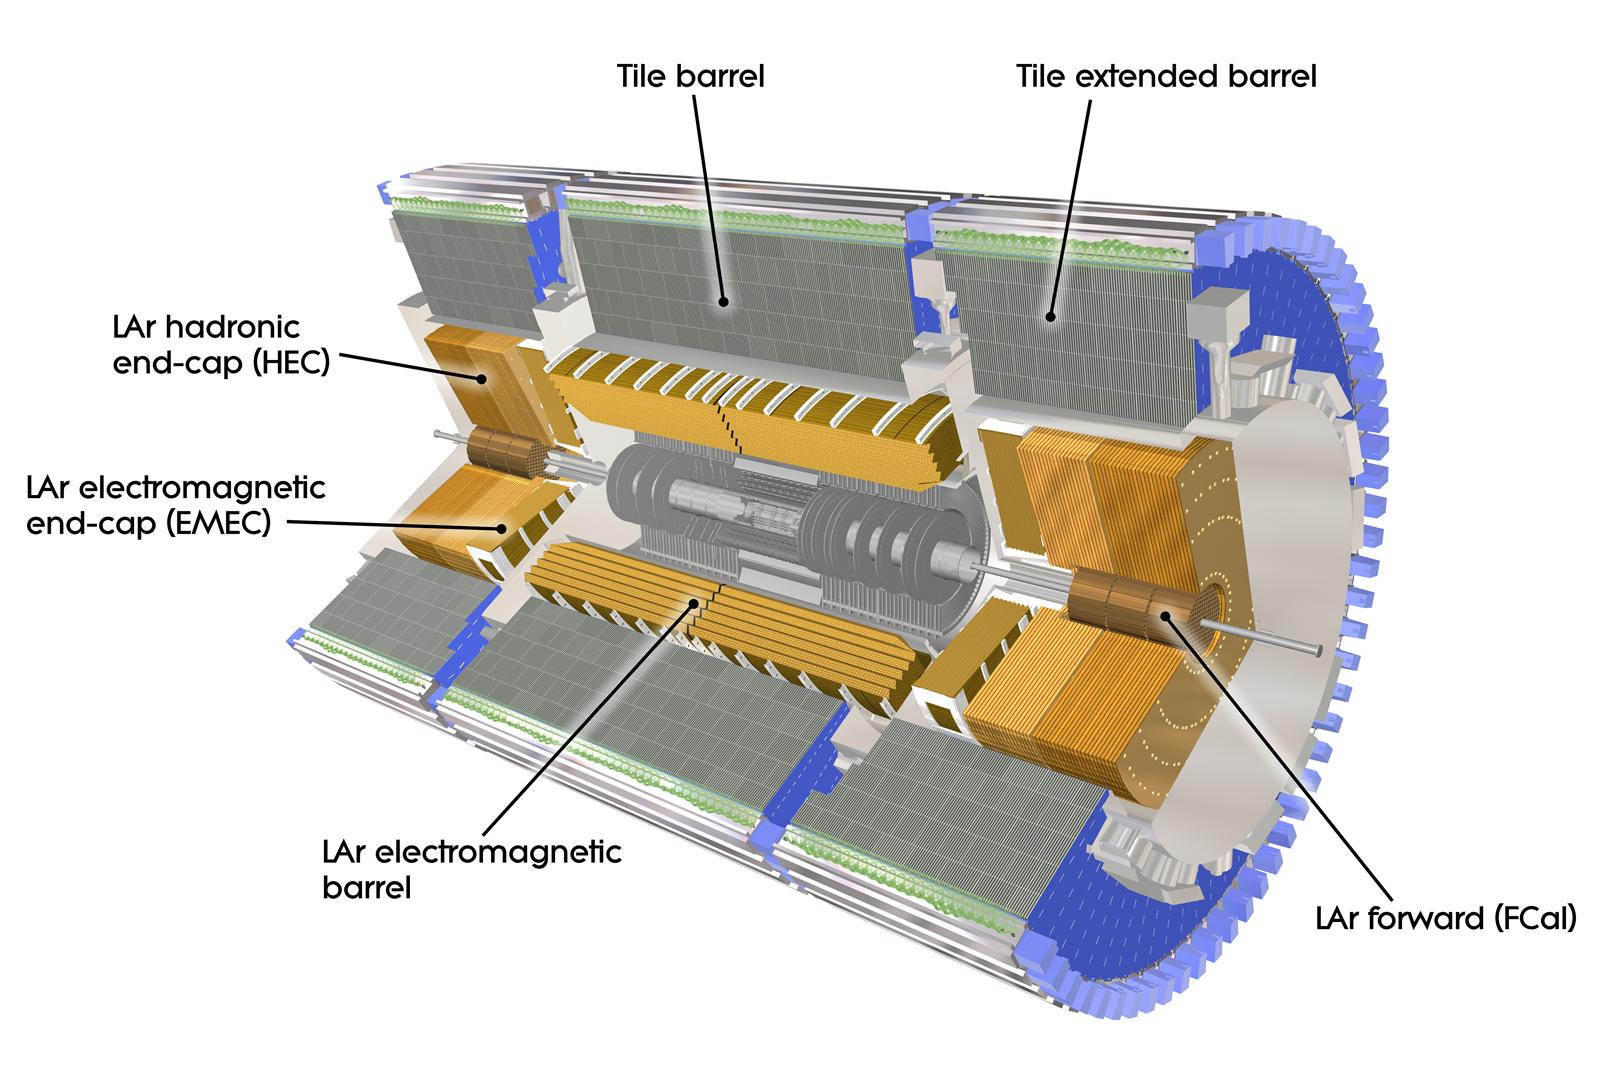
\includegraphics[width=0.8\textwidth]{./figures/atlas/calorimeter.jpg}
  \caption[Overview of the ATLAS calorimeter system]{Overview of the ATLAS
    calorimeter system~\cite{calo_fig}.}
  \label{fig:atlas_calo}
\end{figure}

The EM calorimeter is a sampling calorimeter consisting of lead absorbers,
liquid argon (LAr) as the active material with an electrode geometry providing
full azimuthal symmetry. It is divided into a barrel part and two endcaps,
covering~$|\eta| < 1.475$ and $1.375 < |\eta| < 3.2$,
respectively~\cite{atlas_detector}. With the exception of the transition region
between barrel and endcap, $1.35 < |\eta| < 1.5$, and the forward/backward
region, $|\eta| > 2.5$, the LAr EM calorimeter consists of three longitudinal
samplings~\cite{atlas_detector}. The first sampling of the EM calorimeter (EM1),
also called the strip layer, is finely segmented in $\eta$-direction with a
granularity of~$\Delta\eta \times \Delta\varphi = 0.025/8 \times 0.1$ in the
barrel region (excl.\ transition region) and gradually decreasing granularity in
the endcaps. The second and third layer (EM2/EM3) provide a granularity
of~$0.025 \times 0.025$ and~$0.050 \times 0.025$, respectively (excl.\
transition region). An additional active LAr layer precedes the EM calorimeter
in the region~$|\eta| < 1.8$ to correct for energy losses upstream of the
calorimeter system~\cite{atlas_detector}.

For hadron calorimetry the ATLAS experiment uses two different calorimeter types
in the barrel and endcap regions. In the barrel, a sampling calorimeter based on
steel absorbers and plastic scintillating tiles, the so called tile calorimeter,
is used. It is separated into a barrel part, $|\eta| < 1.0$, and two extended
barrels, $0.8 < |\eta| < 1.7$ (cf.\ Figure~\ref{fig:atlas_calo}). Similar to the
LAr EM calorimeter, it the tile calorimeter is segmented into three longitudinal
samplings. The lateral segmentation of these layers is~$0.1 \times 0.1$ in the
first two layers and~$0.2 \times 0.1$ in the last layer~\cite{atlas_detector}.
The Hadronic Endcap Calorimeter (HEC), located behind the LAr EM endcaps, uses
copper absorbers and LAr as the active material. The HEC provides a
pseudorapidity coverage of $1.5 < |\eta| < 3.2$, partially overlapping the tile
extended barrel, with two longitudinal samplings. The granularity in the region
of high-precision physics measurements, $|\eta| < 2.5$, is $0.1 \times 0.1$.

\subsection{Topological Cell Clustering}

In the ATLAS experiment a topological cell clustering algorithm is used to
reconstruct three-dimensional energy depositions in the calorimeter system,
while suppressing noise from calorimeter cells not topologically connected to
cells with significant signal strength. The TopoCluster
algorithm~\cite{atlas_topoclustering} used in the ATLAS experiment operates on
individual cells of the calorimeter calibrated at electromagnetic energy scale,
therefore not accounting for the different calorimeter response to hadronic
showers. The cluster formation is seeded by the cell of largest signal
significance~\cite{atlas_topoclustering}
\begin{align*}
  \varsigma_\text{cell}^\text{EM} = \frac{E_\text{cell}^\text{EM}}{\sigma_\text{noise,cell}^\text{EM}} \eqcomma
\end{align*}
where~$E_\text{cell}^\text{EM}$ is the cell signal
and~$\sigma_\text{noise,cell}^\text{EM}$ the estimated noise of the cell, if it
passes a seed threshold of~$|\varsigma_\text{cell}^\text{EM}| > 4$. The cluster
is grown by including neighbouring cells in the same and adjacent layers of the
calorimeter that pass a cell significance threshold
of~$|\varsigma_\text{cell}^\text{EM}| > 2$. If a neighbouring cell is a seed
cell or a cell associated to another cluster passing
the~$|\varsigma_\text{cell}^\text{EM}| > 2$ threshold, both clusters are merged.
The cluster is iteratively grown until the last cell passing
the~$|\varsigma_\text{cell}^\text{EM}| > 2$ has been included. Afterwards, all
adjacent cells are included into the cluster independent of their signal
significance. If a cluster has multiple local maxima, it is split in all three
spatial dimensions to more accurately reflect the substructure of the cluster.
After cluster splitting, cells at the interface of two clusters can be shared
between them according to an assigned weight~$w_\text{cell}$ to each cluster.

The geometrical shape and distribution of cell signals in a TopoCluster is
characterised by so called cluster moments. The $n$-th moment of a cell
variable~$v_\text{cell}$ is given by \cite{atlas_topoclustering}
\begin{align*}
  \langle v_\text{cell}^n \rangle = \frac{\sum_{i \mid E_{\text{cell,}i}^\text{EM} > 0} w_{\text{cell,}i} \, E_{\text{cell,}i}^\text{EM} \, v_{\text{cell,}i}^n}{\sum_{i \mid E_{\text{cell,}i}^\text{EM} > 0} w_{\text{cell,}i} \, E_{\text{cell,}i}^\text{EM}} \eqdot
\end{align*}
An example of a cluster moment is the first moment of the Cartesian coordinates
of a cell centre, defining the barycentre of a cluster. An example for a signal
moment is the signal density given by $\langle \rho_\text{cell} \rangle$, where
$\rho_\text{cell} = E_\text{cell} / V_\text{cell}$ is the energy density in a
given calorimeter cell.

\subsection{Local Hadronic Calibration}
\label{sec:local_hadronic_calib}

The calorimeters of the ATLAS detector are non-compensating, that is the
calorimeter response is different for electromagnetic and hadronic showers
originating from particles of the same energy. The local hadronic calibration
(LC), described in Ref.~\cite{atlas_topoclustering}, provides a calibration for
clusters reconstructed with the TopoCluster algorithm without prior assumption
of the particle that created it. The LC scale accounts for the non-compensating
nature of the calorimeters, out-of-cluster energy and dead
material~\cite{atlas_topoclustering}.

The calibration procedure starts with clusters at the electromagnetic energy
scale. Cluster moments determined by the TopoCluster algorithm allow to
discriminate between electromagnetic and hadronic showers. Depending on a
likelihood~$\mathcal{P}_\text{clus}^\text{EM}$, characterising the probability
for a cluster to originate from an electromagnetic shower, a calibration factor
for hadronic showers is applied to the cluster to correct the non-compensating
nature of the calorimeter response. Additional calibrations factors are applied
to account for signal loss due to cells being omitted from the cluster due to
the noise suppression of the TopoCluster algorithm and dead material.

%%% Local Variables:
%%% mode: latex
%%% TeX-master: "mythesis"
%%% End:
